\documentclass[12pt]{article}

%% FONTS
%% To get the default sans serif font in latex, uncomment following line:
 \renewcommand*\familydefault{\sfdefault}
%%
%% to get Arial font as the sans serif font, uncomment following line:
%% \renewcommand{\sfdefault}{phv} % phv is the Arial font
%%
%% to get Helvetica font as the sans serif font, uncomment following line:
% \usepackage{helvet}
\usepackage[small,bf,up]{caption}
\renewcommand{\captionfont}{\footnotesize}
\usepackage[left=1in,right=1in,top=1in,bottom=1in]{geometry}
\usepackage{graphics,epsfig,graphicx,float,subfig,color}
\usepackage{amsmath,amssymb,amsbsy,amsfonts,amsthm}
\usepackage{url}
\usepackage{boxedminipage}
\usepackage[sf,bf,tiny]{titlesec}
 \usepackage[plainpages=false, colorlinks=true,
   citecolor=blue, filecolor=blue, linkcolor=blue,
   urlcolor=blue]{hyperref}
\usepackage{enumitem}
\usepackage{multirow}

\newcommand{\todo}[1]{\textcolor{red}{#1}}
% see documentation for titlesec package
% \titleformat{\section}{\large \sffamily \bfseries}
\titlelabel{\thetitle.\,\,\,}


\newcommand{\bs}{\boldsymbol}
\newcommand{\alert}[1]{\textcolor{red}{#1}}
\setlength{\emergencystretch}{20pt}

\begin{document}

\begin{center}

\large \textbf{%%
High Performance Computing \\ Assignment \#4 \\ Yuan-Xun Bao \\ yxb201@nyu.edu \quad N13392943}
\end{center}

% ****************************
\section{Part (a)}

\begin{figure}[h]
\centering
\subfloat[][Original image, size: 1280$\times$720]{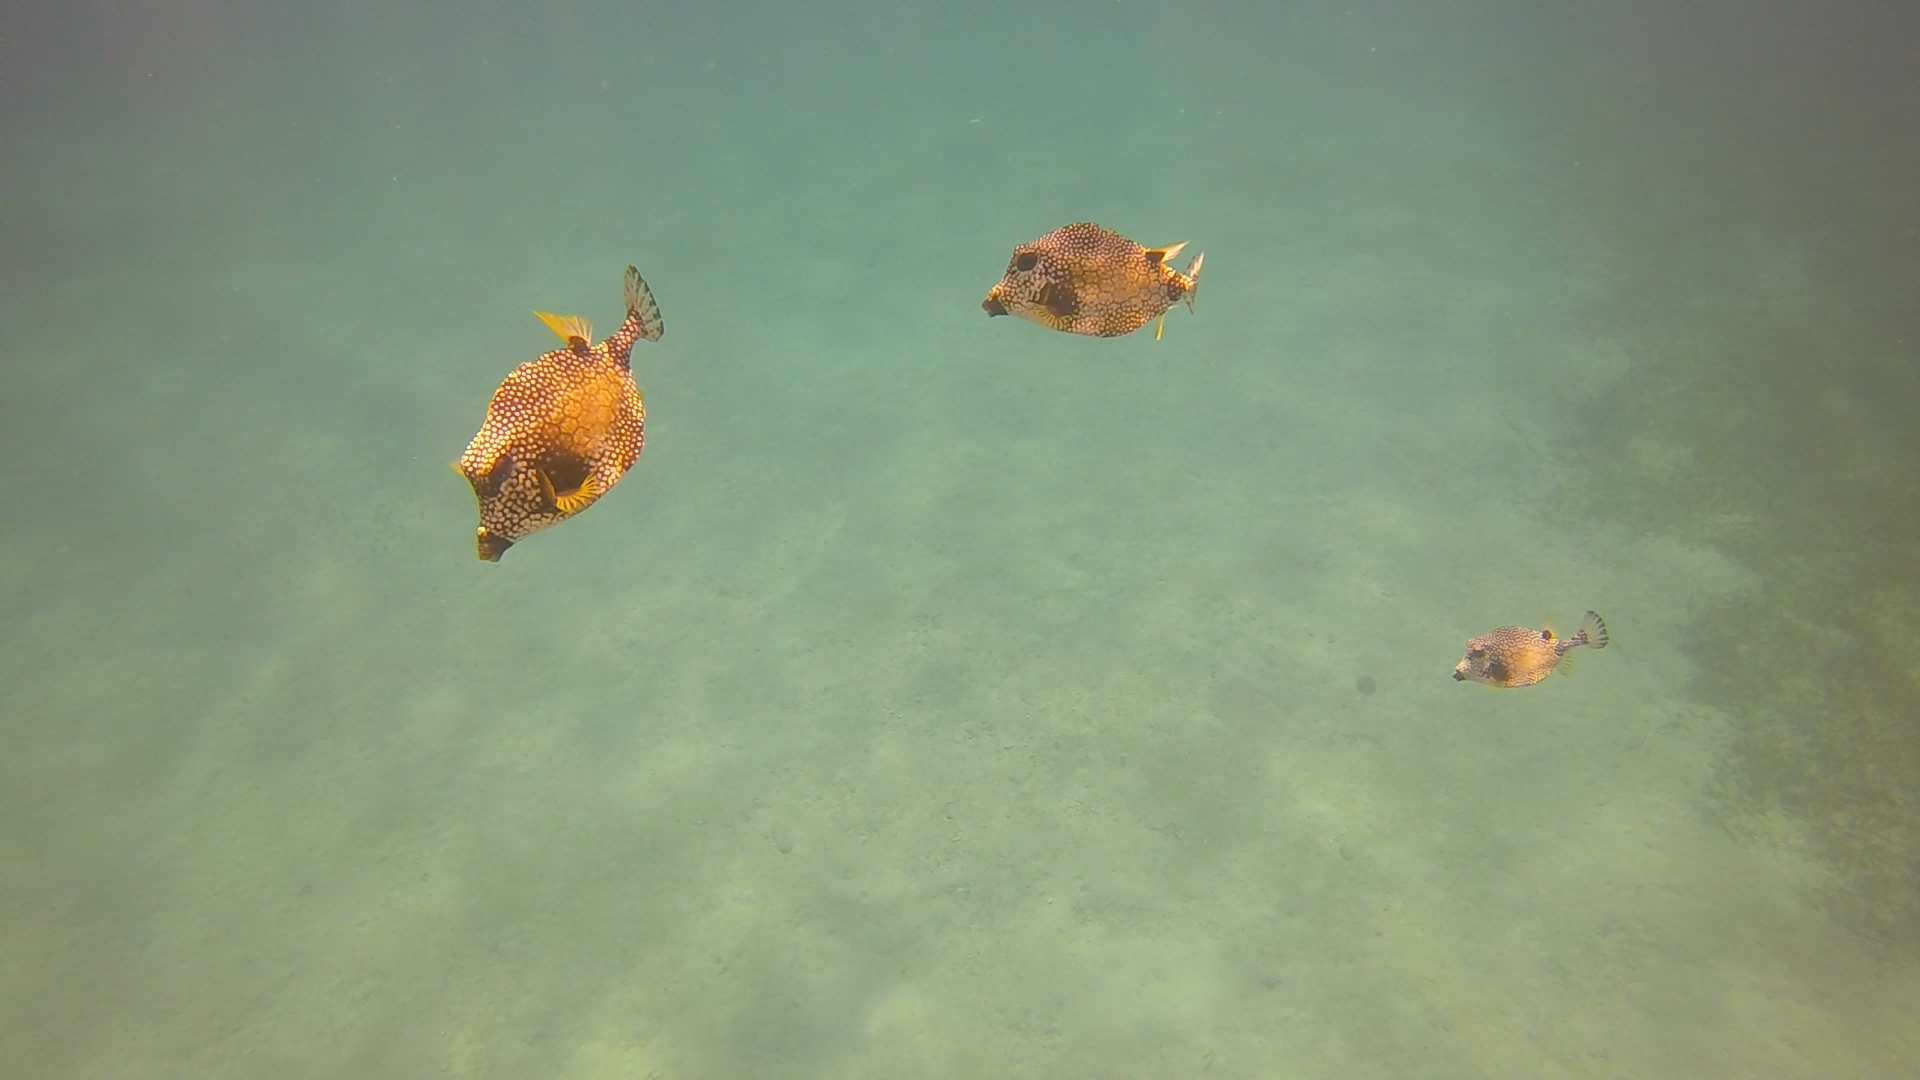
\includegraphics[width = .8\linewidth]{fish.jpg}} \\
\subfloat[][Output image after 1 iteration of blurring]{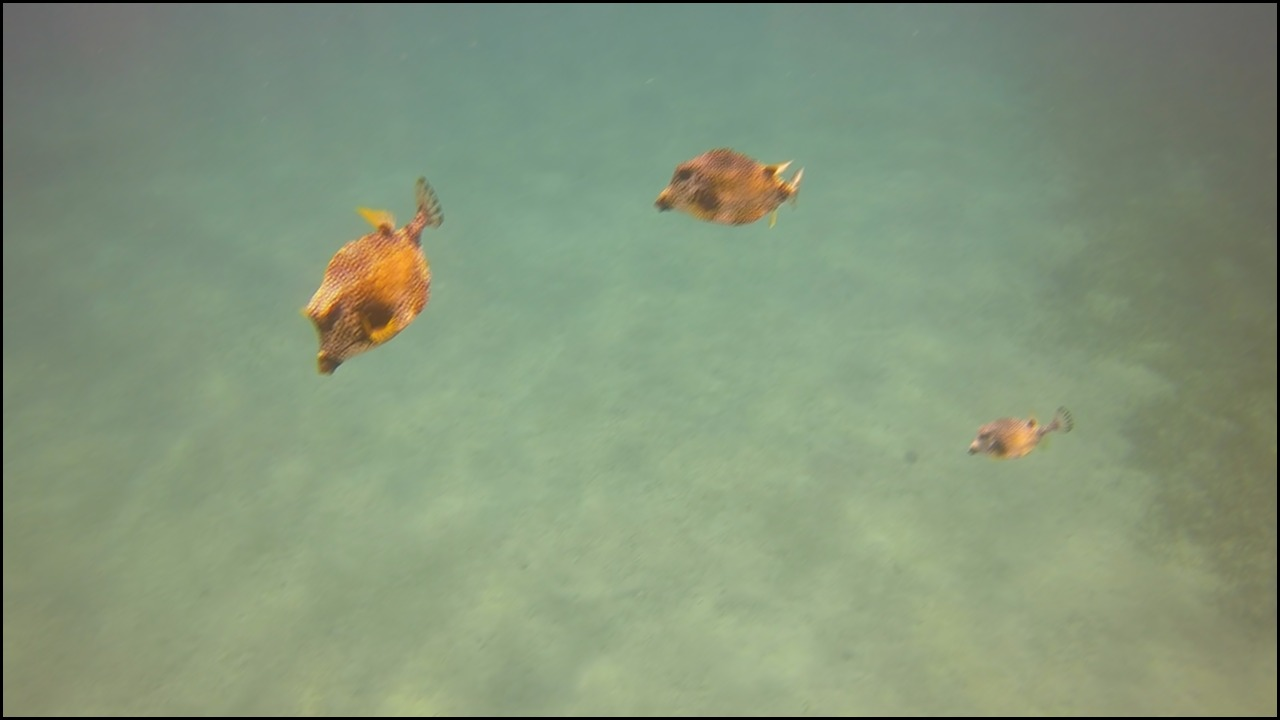
\includegraphics[width = .8\linewidth]{blur1.jpg}}
\caption{run repeatedly 100 times, 16$\times$16 workitems}
\end{figure}

\begin{table}[h]
  \centering
  \begin{tabular}{ | c | c | c | c | c |}
    \hline
    GPU/CPU model & Total time (s) & MPixels/s & GBits/s & GFlops/s \\ \hline
     Intel(R) Core(TM)  & \multirow{2}{*}{0.172978} & \multirow{2}{*}{5.327835} & \multirow{2}{*}{0.170491}  & \multirow{2}{*}{1.037467}  \\ 
     i3-2120 CPU @ 3.30GHz & & & & \\ \hline
     GeForce GTX  & \multirow{2}{*}{0.001586} & \multirow{2}{*}{581.255344} & \multirow{2}{*}{18.600171} & \multirow{2}{*}{113.185453} \\ 
     TITAN Black & & & &  \\ \hline
    AMD &  \multirow{2}{*}{0.004423} &  \multirow{2}{*}{208.345356} &  \multirow{2}{*}{6.667051}  &  \multirow{2}{*}{40.570231} \\
    Cypress & & & & \\ \hline
    NVIDIA & \multirow{2}{*}{0.006643} & \multirow{2}{*}{138.730690} & \multirow{2}{*}{4.439382} & \multirow{2}{*}{27.014454} \\
    Tesla T10 & & & & \\ \hline
  \end{tabular}
    \caption{Run repeatedly 100 times, 16$\times$16 workitems}
\end{table}

As a result of increasing the number of workitems, the performance on GPU decreases but the increases on CPU. 
\begin{table}[h]
  \centering
  \begin{tabular}{ | c | c | c | c | c |}
    \hline
    GPU/CPU model & Total time (s) & MPixels/s & GBits/s & GFlops/s \\ \hline
     Intel(R) Core(TM)  & \multirow{2}{*}{0.029974} & \multirow{2}{*}{30.746817} & \multirow{2}{*}{0.983898}  & \multirow{2}{*}{5.987200}  \\ 
     i3-2120 CPU @ 3.30GHz & & & & \\ \hline
     GeForce GTX  & \multirow{2}{*}{0.002282} & \multirow{2}{*}{403.932833} & \multirow{2}{*}{12.925851} & \multirow{2}{*}{78.656173} \\ 
     TITAN Black & & & &  \\ \hline
    \end{tabular}
    \caption{Run repeatedly 100 times, 32$\times$32 workitems}
\end{table}
%  \multirow{2}{*}{}

\newpage

\section{Part (b)}
\begin{figure}
\centering
\subfloat[][Output image after blurring recursively 100 times]{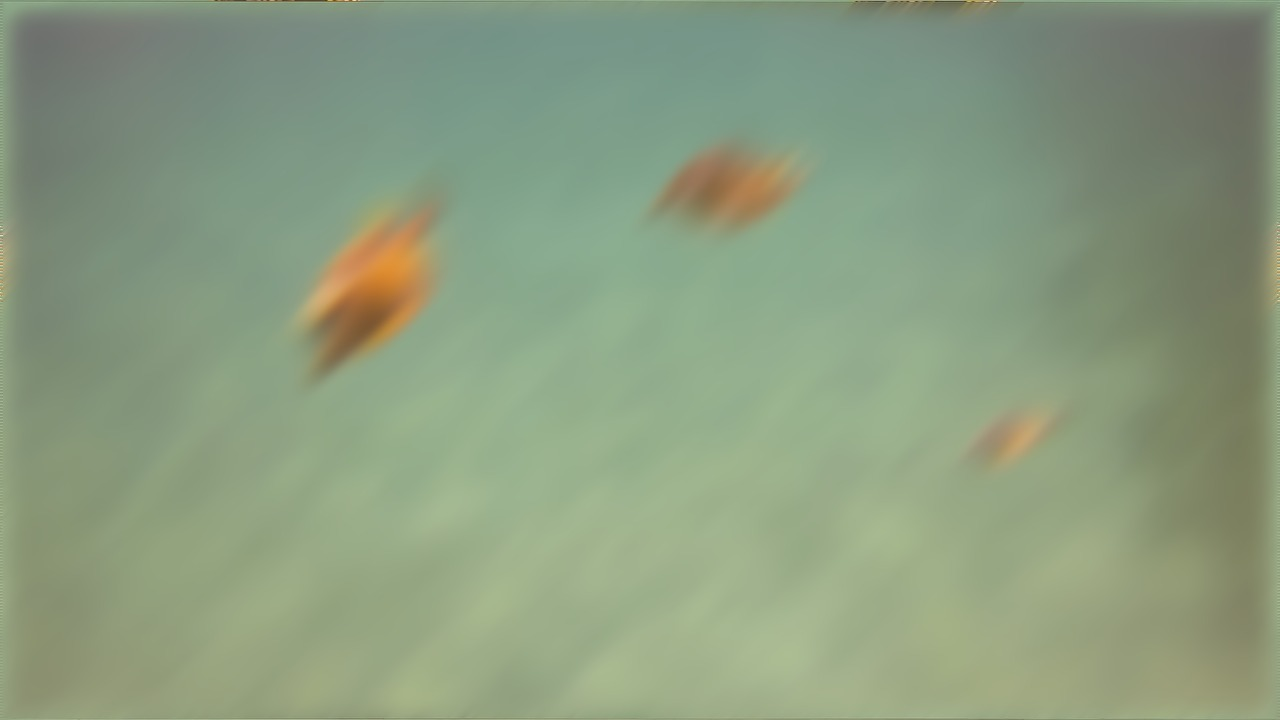
\includegraphics[width = .7\linewidth]{blur100.jpg}} \\
\subfloat[][Output image after blurring recursively 200 times]{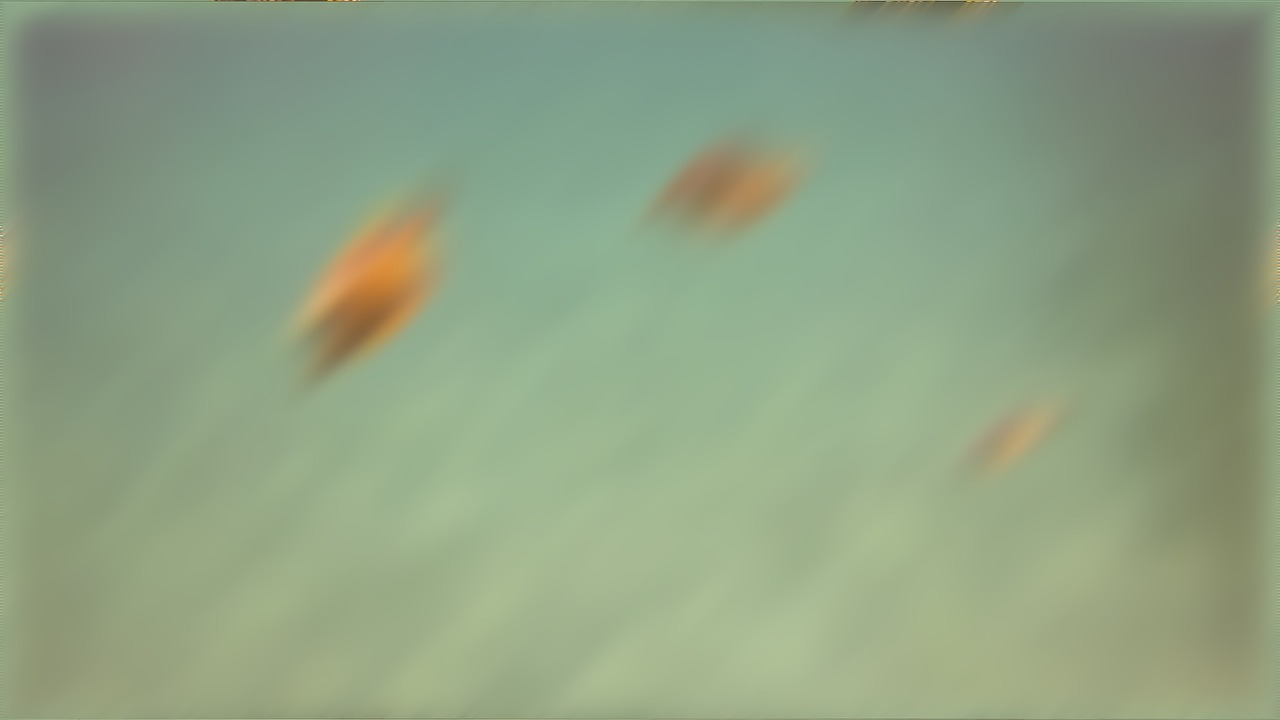
\includegraphics[width = .7\linewidth]{blur200.jpg}}\\
\subfloat[][Output image after blurring recursively 300 times]{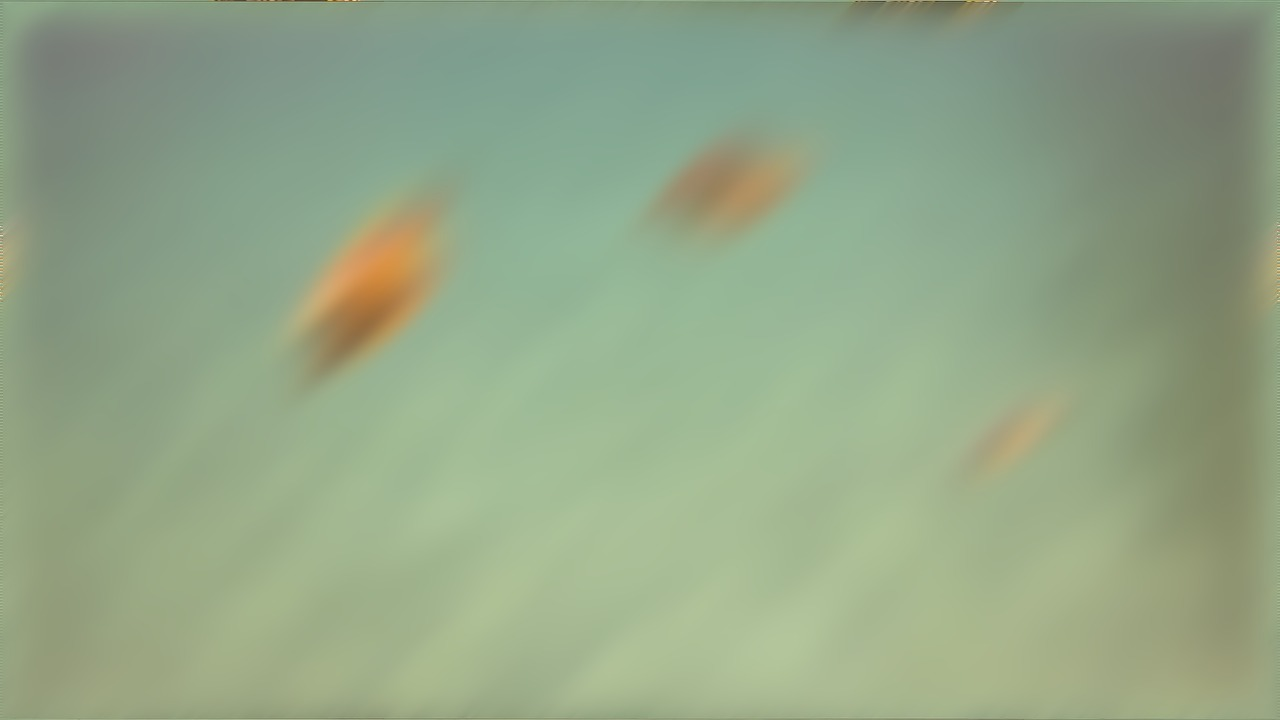
\includegraphics[width = .7\linewidth]{blur300.jpg}}\\
\caption{run iterative 100, 200, 300 times, 16$\times$16 workitems}
\end{figure}

\end{document}
